\documentclass[onecolumn]{IEEEtran}

\usepackage[left=1.5cm,right=1.5cm]{geometry}
\usepackage[
spanish,
es-nodecimaldot,
es-tabla
%english
]{babel}
\usepackage[utf8]{inputenc}
\usepackage[T1]{fontenc}
\usepackage{float}
\usepackage{crossreftools}
\usepackage{graphicx}
\usepackage{grffile}
\usepackage{longtable}
\usepackage{wrapfig}
\usepackage{rotating}
\usepackage[normalem]{ulem}
\usepackage{amsmath}
\usepackage{textcomp}
\usepackage{amssymb}
\usepackage{capt-of}
\usepackage{hyperref}
\usepackage{minted}
\usepackage{subfiles}
\usepackage{caption}
\usepackage{subcaption}
\usepackage[acronym, toc]{glossaries}


\usepackage{fancyhdr}
\usepackage{graphicx}
\usepackage[table,xcdraw]{xcolor}
\usepackage{multicol}
\usepackage{tabularx,booktabs}
\usepackage{siunitx}

\usepackage{grffile}
\usepackage{longtable}
\usepackage{rotating}
\usepackage[normalem]{ulem}
\usepackage{amsmath}
\usepackage{textcomp}
\usepackage{amssymb}
\usepackage{capt-of}
\usepackage{booktabs}
\usepackage{hyperref}
\usepackage{caption}

\definecolor{LightGray}{gray}{0.9}
\definecolor{DarkGray}{HTML}{191919}
\definecolor{custom}{HTML}{F8F8F8}

\newenvironment{code}{\captionsetup{type=listing}}{}

\usemintedstyle{emacs}

\usepackage[ruled,vlined]{algorithm2e}


\renewcommand{\listingscaption}{Código}
\renewcommand\listoflistingscaption{Índice de \listingscaption\@s}

\setminted[python]{frame=single,framesep=3mm,baselinestretch=0.9,breaklines=true,bgcolor=custom,fontsize=\scriptsize,linenos}
\setminted[shell-session]{frame=single,framesep=1mm,baselinestretch=0.5,breaklines=true,bgcolor=custom,fontsize=\scriptsize}
\graphicspath{
  {./img_common}
  {./img}
}
% \usepackage[T1]{fontenc}
% \renewcommand*\familydefault{\sfdefault} %% Only if the base font of the document is to be sans serif

% \pagestyle{fancy}
% \fancyfoot[R]{\thepage}
% \fancyfoot[C]{\includegraphics[width=0.05\textwidth]{inge_logo}}
% \fancyhead[L]{\leftmark}
% \fancyhead[R]{\rightmark}


\usepackage{authblk}
\usepackage[backend=biber,style=ieee]{biblatex}
\addbibresource{./main.bib}

\begin{document}

\begin{titlepage}
  \centering
  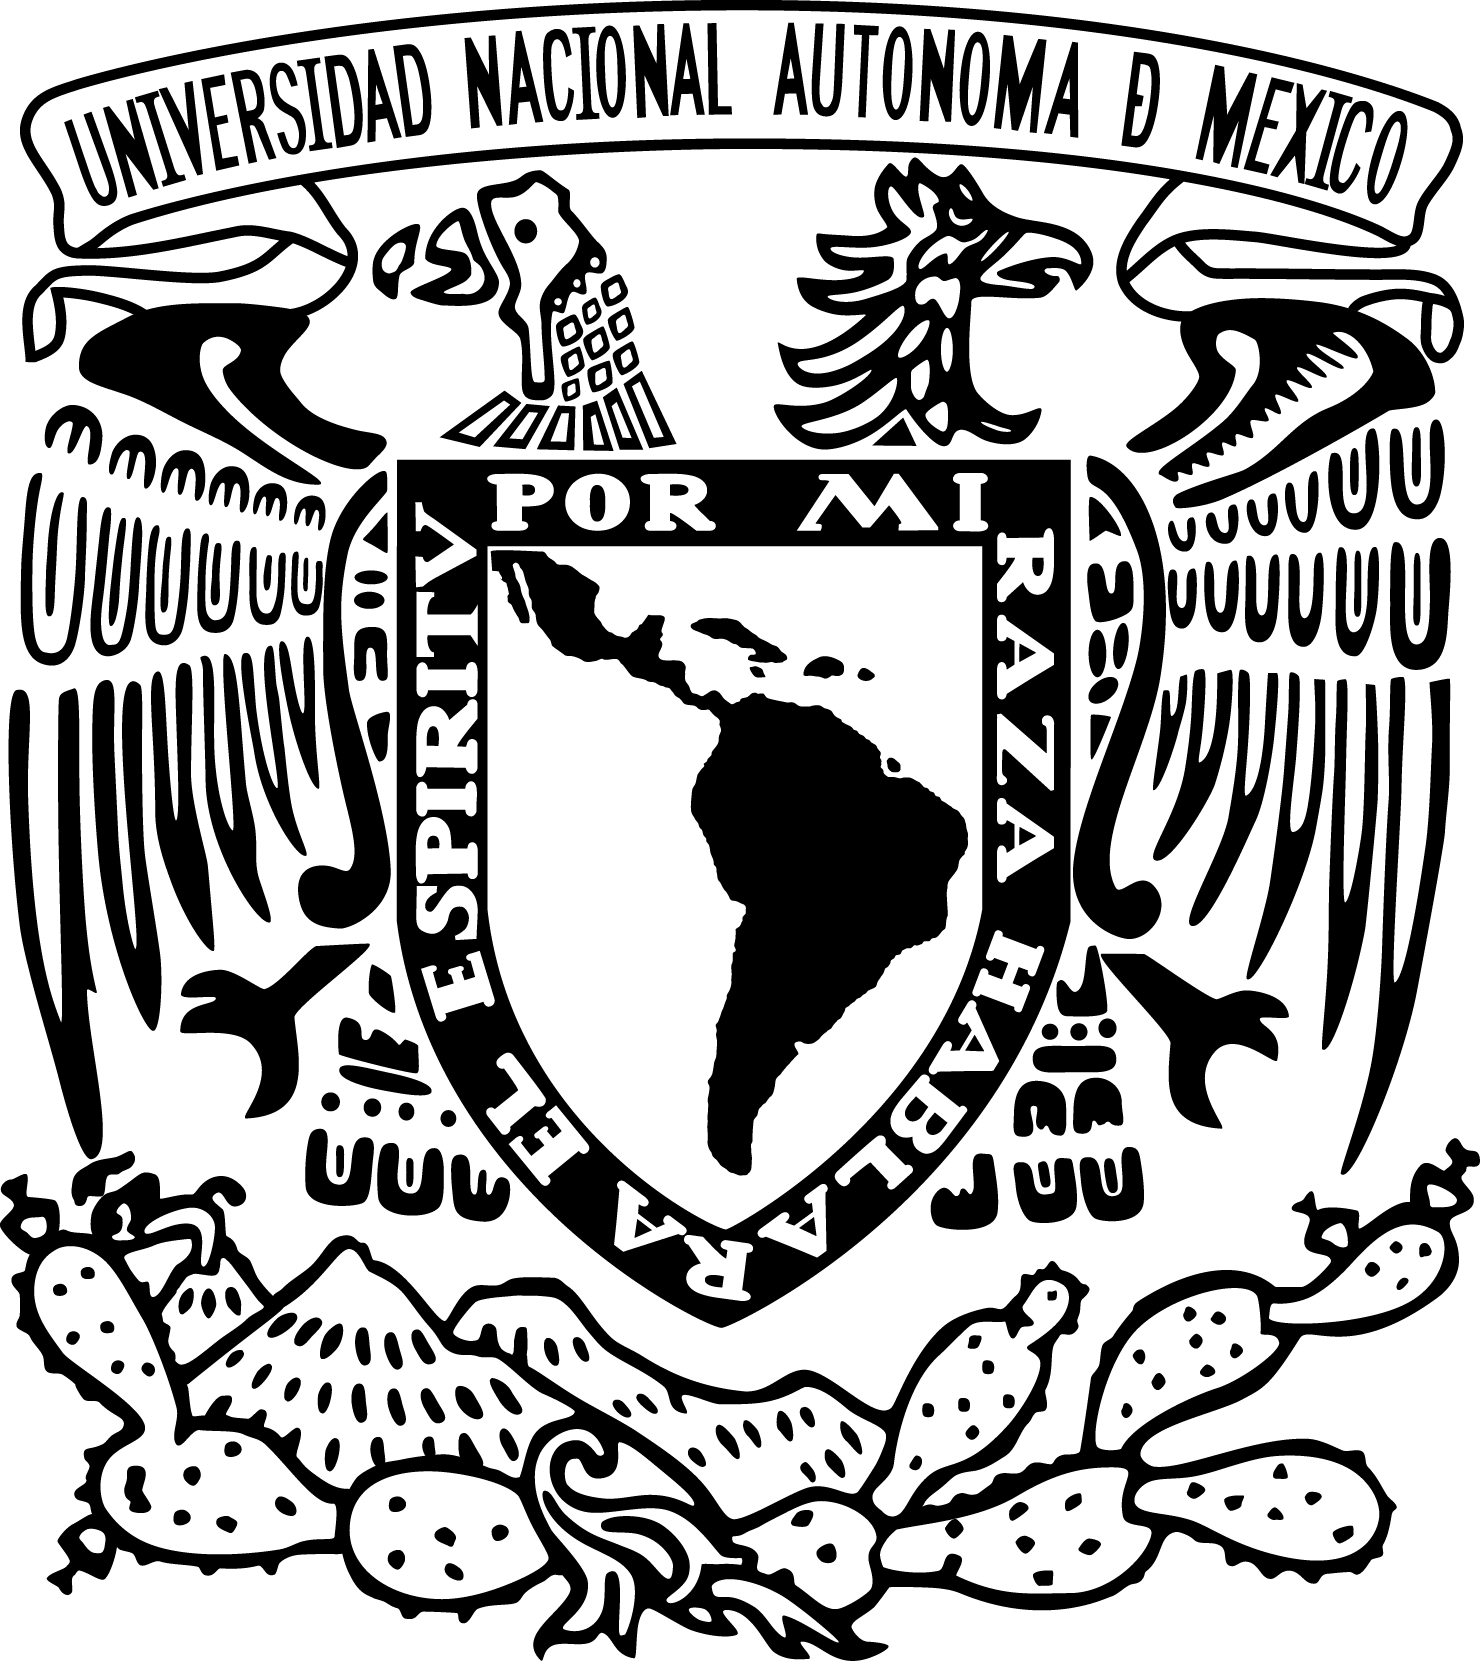
\includegraphics[width=0.3\textwidth]{unam-escudo}\vfill{}
  \Huge{Facultad de Ingeniería}\\
  \huge{Criptografía}\vfill{}
  \Huge{Proyecto Final}
  \\
  \vfill{}
  \LARGE{Alumnos:}
  \begin{flushleft}
    \begin{itemize}
      \item Machicao Cardoso Raúl Fernando
      \item Martínez López Andrés
      \item Romero Andrade Cristian
      \item Romero Andrade Vicente
    \end{itemize}
  \end{flushleft}
  \vfill{}
  % \Large{Grupo: 6}\\
  \Large{Semestre 2021--2}
  \vfill{}
  \LARGE{Profesora: Dra.~Rocio Alejandra Aldeco Perez}
  \vfill
  % \Large{Fecha de entrega: 14 de junio de 2021}
  % \vfill
  
\includegraphics[width=0.1\textwidth]{fi_logo}
\end{titlepage}


\title{Proyecto Final}
\author{
  \IEEEauthorblockN{
    Romero Andrade Cristian\IEEEauthorrefmark{1},
    Romero Andrade Vicente\IEEEauthorrefmark{2},
    Machicao Cardoso Raúl Fernando\IEEEauthorrefmark{3} y
    Martínez López Andrés\IEEEauthorrefmark{4}
  }
  \IEEEauthorblockA{Criptografía,
    Facultad de Ingeniería\\
    Email: \IEEEauthorrefmark{1}\href{mailto:cristian.romero@comunidad.unam.mx}{cristian.romero@comunidad.unam.mx},
    \IEEEauthorrefmark{2}\href{mailto:dark_reggae_93@comunidad.unam.mx}{dark\_reggae\_93@comunidad.unam.mx},
    \IEEEauthorrefmark{3}\href{mailto:laastar@comunidad.unam.mx}{laastar@comunidad.unam.mx},
    \IEEEauthorrefmark{4}\href{mailto:bockerlaila@comunidad.unam.mx}{bockerlaila@comunidad.unam.mx}}}

\maketitle{}

\tableofcontents{}

\subfile{./secciones/introduccion.tex}

\newpage{}

\subfile{./secciones/desarrollo.tex}

\clearpage{}

\section{Conclusiones}\label{sec:concluciones}
Para el presente trabajo comparamos varios algoritmos desde AES, pasando por SHA hasta las de curva elíptica como ECDSA, cada uno para una o unas tareas específicas. En principio al entender que cada uno de estos algoritmos se enfocan en diferentes objetivos los cuales podemos definir en tres métodos principales como 1) Cifrado y descifrado; 2) Hashing; y 3) Firma y Verificación, es como podemos entender y realizar las pruebas necesarias para evaluar que tan eficaces son dichos algoritmos.

Empezando por el método de Cifrado y Descifrado, tenemos a los algoritmos AES, los cuales en esta ocasión tenemos a AES-CBC y AES-ECB los cuales fueron puestos a prueba con algunos de los tipos de archivo más comunes (vectores, pdf, imagen y zip) en la cual se observó que el algoritmo AES-CBC tanto para cifrar como descifrar tarda más tiempo que el de AES-ECB, lo cual nos indica que este ultimo sacrifica seguridad para obtener una respuesta de cálculo más rápida.

Siguiendo dentro del mismo método, tenemos a los algoritmos RSA-OAEP, los cuales fueron puestos a prueba con 20 vectores para tener una muestra significativa que pudiera arrojarnos un resultado confiable, dichos vectores fueron conformados por un modulo y un exponente privado (llave privada) de gran tamaño; un exponente público (llave pública) de tamaño pequeño; y el dato de tamaños variables para cada uno de dichos vectores. Así, de esta manera observamos que tanto para el cifrado como descifrado logran mantener un tiempo relativamente constante, en donde se lleva mayor tiempo descifrar, lo cual nos indica que estos algoritmos son mucho más estables y ofrecen una mayor seguridad a los AES, ya que en el tiempo es directamente proporcional al cifrar y descifrar, aunque cabe destacar que es más lento.

Pasando al método de Hashing tenemos a los algoritmos SHA-2 (384 y 512 bits) y SHA-3 (384 y 512 bits), los cuales fueron probados con los mismos archivos que en AES, en donde es observable que los algoritmos SHA-2 son más rápidos que los SHA-3, y del mismo modo, son más rápidos los de 384 bits que los de 512 bits. Sin embargo, como se mencionó anteriormente el SHA-3 se puede implementar a través de hardware, por lo que entonces el SHA-3 puede ser igual de rápido e incluso más rápido que el SHA-2.

Teniendo finalmente el método de Firma y Verificación con los algoritmos RSA-PSS, DSA y ECDSA (Prime field y Binary field), dichos algoritmos al igual que con los RSA-OAEP, fueron puestos aprueba con 20 vectores formados como se mencionó anteriormente, con lo cual de manera general fue observable que para los algoritmos que no implican curvas elípticas (todos excepto los ECDSA) verificar el dato es más rápido que firmarlo, así mismo el tiempo de verificación para RSA-PSS y DSA es prácticamente el mismo, mientras que para la firma es más rápido el DSA. Pasando a los algoritmos ECDSA observamos que la firma es más rápida que la verificación (siendo más lento los del campo binario), lo cual nos indica que efectivamente el uso de curvas elípticas garantiza una mayor seguridad en comparación a los algoritmos que utilizan exponenciaciones.

Una vez analizado los diferentes algoritmos en este trabajo, podemos decir que, si bien algunos de estos algoritmos destacan en su velocidad, no cabe duda que pueden llegar a sacrificar robustez (tal como pasó con SHA–1 en su momento). Unos algoritmos son más nuevos que otros, por lo cual los más recientes tienen ciertos antecedentes que benefician para su diseño teniendo una excelente relación velocidad—seguridad.

En conclusión, los diversos tipos de algoritmos ofrecen diferentes características las cuales dependiendo de lo que busquemos, ya sea mayor velocidad, mayor seguridad, mayor veracidad, etc. Es como debemos elegirlos y aplicarlos, ya que debemos buscar lo que nos de mayor eficiencia posible sin arriesgar tanto, es por eso que como se observó en el presente trabajo, para cada tipo de archivo que nosotros encriptemos o firmemos corresponderá al tiempo en el que se descifra o verifica el archivo, de esta forma con las pruebas realizadas y con los diferentes parámetros con los que se probaron los algoritmos AES, RSA, SHA-2, SHA-3, DSA y ECDSA es como podemos optar por un método de encriptación que nos garantice la autenticidad de nuestros archivos.


\nocite{*}

\newpage{}

\listoffigures{}
\listoftables{}
\listoflistings{}

\addcontentsline{toc}{section}{Referencias}
\printbibliography{}

\end{document}
